\chapter[Remote shell FAILED]{The Remote shell mission : \[FAILED\]}
C'est un échec. Alors que je me bats depuis des heures avec le processus ssh, il a gagné (Si j'avais pu faire un dessin d'un processus lourdement armé, je l'aurais mis ici).
\\\\
Cependant il y a quelques directions que j'aurais pu prendre :
\\\begin{itemize}
\item[libssh :] c'est une solution utilisée par d'autres étudiants. Si le moral revient après ma défaite, j'explorerai cette possibilité (même si je considère tout de même qu'il s'agit, en quelque sorte, d'un court-circuit du projet) ;
\item[ssh <serv> <cmd> :] s'il n'y a pas d'authentification, je peux lancer les commandes isolées. C'est pas très propre, puisqu'il faut relancer la connexion en permanence ;
\item[ssh <serv> bash :] encore une solution utilisée par d'autres étudiants. C'est une sorte d'amélioration de la précédente. Elle a l'avantage de conserver la connexion. Elle outrepasse aussi un problème : elle permet de continuer à interagir avec notre processus. Après un exec(), à moins qu'il y ait une erreur, on ne peut plus rien faire.
\\\end{itemize}
Je pense qu'une fois l'authentification passée, le mieux est de lier un terminal à chaque processus, que ce soit en entrée ou en sortie. Le programme principal conserve un droit d'écriture dans l'entrée standard de ces processus ssh. Ça a l'avantage d'agir comme si chaque terminal s'était connecté indépendamment, mais le tout lancé via un seul, et aussi de pouvoir tout de même lancer des commandes via le principal, voir même lancer des commandes à tous (on pourrait sans difficulté créer une commande "remote send <serv1> <serv2>..." qui demande ensuite une commande, et l'envoie à ces serveurs précis). Il y aurait moyen de faire des choses sympas, et pratiques.
\\Je regarde libssh, et ça simplifie énormément la chose. Dans un sens, traiter une commande interne avec des fonctions C, c'est plus logique, mais bon. C'est avec cette librairie qu'il fallait sûrement partir. Même les autres solutions me semblent trop archaïques pour que ce soient celles attendues. L'authentification est de plus possible avec libssh. Il suffit de le demander sur le terminal, sans l'afficher, et de l'envoyer à ssh\_userauth\_password().
\\\\
\textbf{> Failure}
\\\\
Quelques ajustements avant de procéder au dernier push de ce projet. Je confirme que remote ne sera pas fait. Les \#include inutiles ont été retirés. Vous trouverez d'ailleurs sur la page suivante un schéma de dépendance des fichiers locaux.
\\C'est ici que ce terminent ce projet, et ce rapport.
\\\\
\textbf{> The End}
\newpage
\begin{figure}[p]
\centering
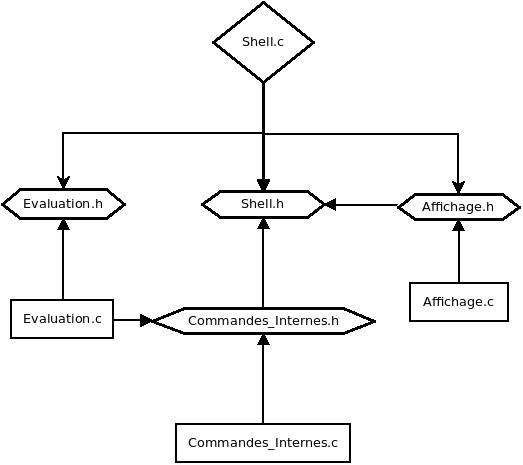
\includegraphics[width=400pt]{Diagramme_dependances.jpg}
\caption{Schéma de dépendance des fichiers locaux de ce projet}
\end{figure}